%% Commands for TeXCount
%TC:macro \cite [option:text,text]
%TC:macro \citep [option:text,text]
%TC:macro \citet [option:text,text]
%TC:envir table 0 1
%TC:envir table* 0 1
%TC:envir tabular [ignore] word
%TC:envir displaymath 0 word
%TC:envir math 0 word
%TC:envir comment 0 0

\documentclass[sigplan,screen]{acmart}
%% \BibTeX command to typeset BibTeX logo in the docs
\AtBeginDocument{%
  \providecommand\BibTeX{{%
    Bib\TeX}}}

\usepackage{pgfplots}
\pgfplotsset{compat=1.18}
\usepackage{array}
\usepackage{tabularx}
% Definiert einen neuen Spaltentyp 'L', der die Breite als Argument nimmt
\newcolumntype{L}[1]{>{\raggedright\arraybackslash}p{#1}}
\newcolumntype{Y}{>{\small\raggedright\arraybackslash}X}

\begin{document}

\title{Feasibility of the Ultimate Display}

\author{Arthur Kehrwald}
\email{arthur.kehrwald@smail.th-koeln.de}
\affiliation{%
  \institution{TH Köln}
  \city{Cologne}
  \country{Germany}
}

\begin{abstract}
  This paper assesses the feasibility of the "ultimate display"—an interface visually indistinguishable from a physical window. The most important research in multiview, volumetric, and holographic display technologies is reviewed and evaluated from two different viewpoints: the physical reconstruction of light fields (the plenoptic function) and the satisfaction of human visual perception (depth cues). This analysis demonstrates that multiview systems are most practical, but holographic displays are are better suited as the ultimate display. Finally, the remaining challenges in computational display holography are examined to predict the timescale of further progress.
\end{abstract}

\begin{CCSXML}
<ccs2012>
   <concept>
       <concept_id>10010583.10010786.10010810</concept_id>
       <concept_desc>Hardware~Emerging optical and photonic technologies</concept_desc>
       <concept_significance>300</concept_significance>
       </concept>
 </ccs2012>
\end{CCSXML}

\ccsdesc[300]{Hardware~Emerging optical and photonic technologies}

\keywords{Display technology, Digital holography, Light field, Multiscopic}

\received{26 June 2026}

\maketitle

\section{Introduction}

Apart from displaying abstract information such as text, spreadsheets, and user interfaces, digital display technology aims to faithfully reproduce recorded and synthetic representations of three-dimensional scenes. Most commercial displays are limited to reproducing two-dimensional images on flat, rectangular surfaces. Many specialized display technologies have been developed to address shortcomings of 2D displays for specific applications, but none are capable of producing an image indistinguishable to the naked eye from the object being displayed. This paper aims to rigorously define this idea of an ultimate display and compare it to the state of the art in 3D display research. From this comparison, it should become clear what problems remain unsolved. These challenges are then discussed to assess the technical feasibility and commercial viability of the ultimate display.

\section{Fundamentals}
The properties of the ultimate display follow from human vision. Before discussing display technology, it is therefore necessary to understand exactly why a two-dimensional image of an object looks less convincing than the real thing.
\subsection{Depth perception}
Depth perception is typically analyzed in terms of various contributing factors called depth cues.
\begin{center}
\begin{tabular}{l p{2.5cm} p{2.5cm}}
 & \textbf{Monocular} & \textbf{Binocular} \\ 
 \hline
 \textbf{Visual} & Pictorial cues & Retinal disparity \\  
 \hline
 \textbf{Oculomotor} & Accomodation, Pupillary \par response & Convergence \\
\end{tabular}
\end{center}
Retinal disparity arises from the slight difference in perspective between the left and the right eye. Light originating from the same point in space does not necessarily reach corresponding points on the left and right retinas. A detailed explanation of the geometry is given by Patterson and Martin (1992). \cite{patterson1992human} The oculomotor cues are sensed by proprioceptors in the muscles responsible for focusing the eye lens (Accomodation), turning the eyeballs (Convergence), and constricting as well as dilating the pupil in response to brightness (Pupillary response). The way the eyes adjust in these three ways when viewing an object correlates to its distance. This allows the visual system to use this form of proprioception to perceive depth.
\subsection{The plenoptic function}
\subsection{Light fields}

\section{Definition of the ultimate display}
\label{sec:definition}
\begin{figure}[h]
    \centering
    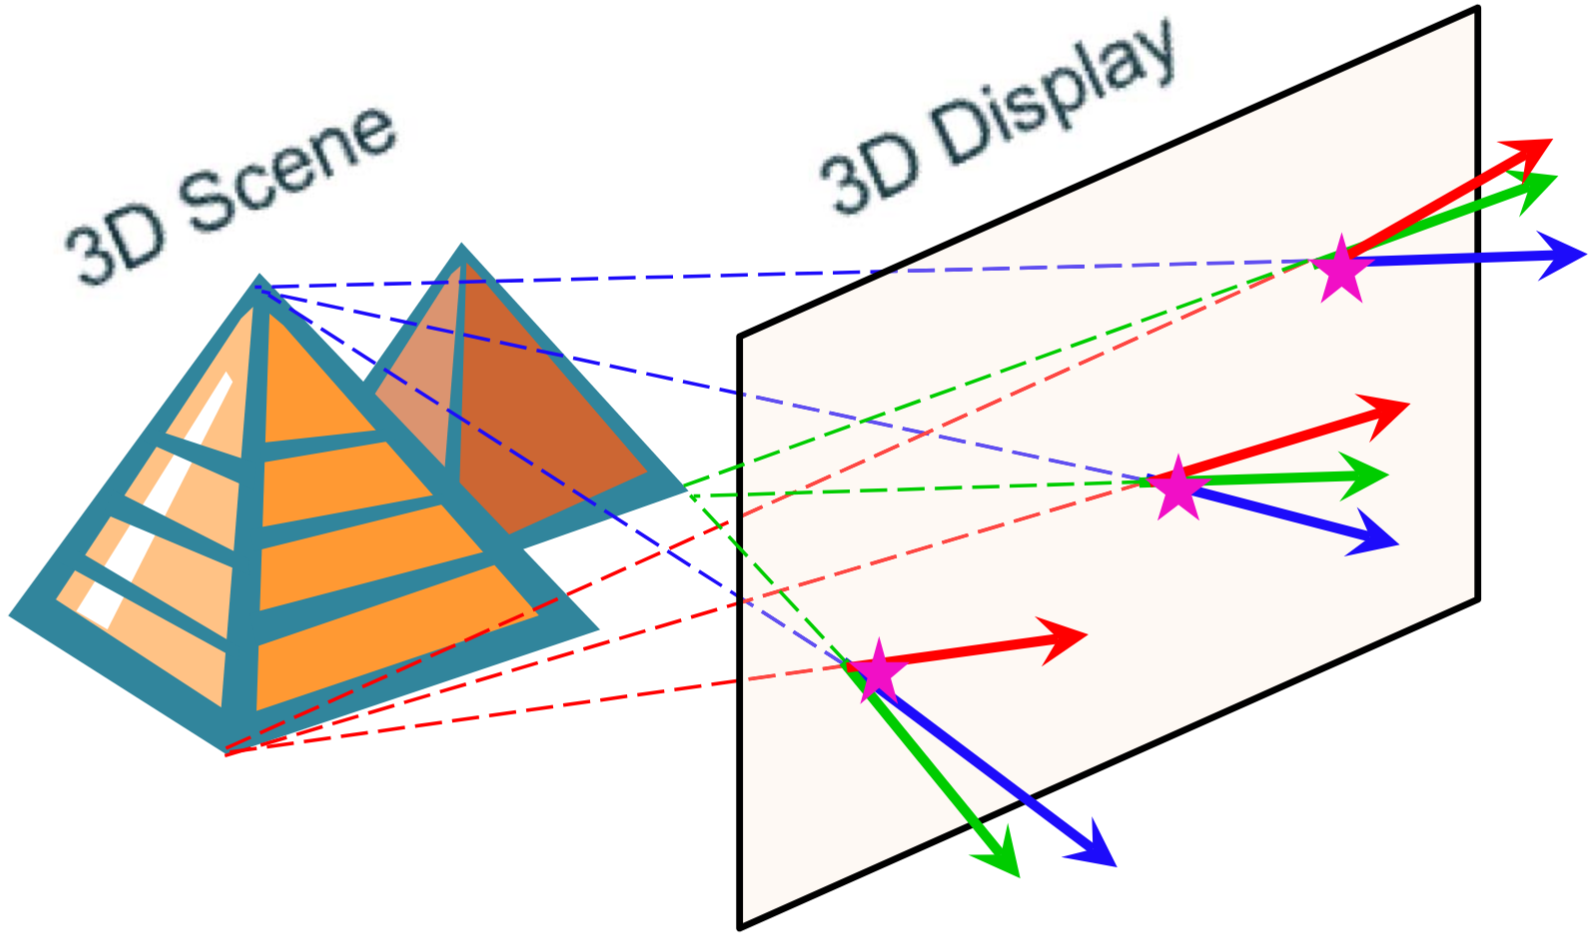
\includegraphics[width=\linewidth]{assets/window}
    \caption{The ultimate display reproduces the position, direction, wavelength, and amplitude of rays from every point of the scene through the display surface. Image from \cite{Geng_2013}}
    \label{fig:window}
\end{figure}

With the background information from the previous sections in mind, the idea of the ultimate display can be further specified. To provide binocular disparity and vergence cues, a display must show a different image to each eye. Motion parallax requires generalizing this feature to provide not just one image per eye, but a continuum of images across the horizontal and vertical axes of the display. Even more challenging is the accommodation cue. If the image should appear sharp at the depths at which its contents are located, the optical elements displaying it must either be spread across a volume themselves or they must be capable of controlling the divergence of the light they emit to mimic point emitters that are not on the display surface. This sounds a lot like displaying a light field, the approach that follows from the idea of approximating the plenoptic function. The key requirement for this is once again to control the direction of light in addition to its wavelength and amplitude. The goal is ultimately to reconstruct the wavefront that would be emitted by the displayed object or scene, thereby producing the "window view upon reality" predicted by Gabriel Lippmann in 1908.\cite{lippmann1908epreuves} In this test or thought experiment, an ideal display would be capable of producing the exact same view simultaneously from every angle that a window would if the displayed scene was really behind it. This requires reproducing the light field at the window plane (fig. \ref{fig:window}). Additionally, it should not require any viewing aids, be agnostic to the number of simultaneous viewers and support some kind of digital interface that clearly separates the optical display hardware from the content. A counterexample would be analog film.

Along the way towards that ideal, many displays have been developed (and some commercialized), that fulfill some of the requirements outlined in the previous section. For this discussion, they will be categorized into multiscopic, volumetric and holographic designs. This taxonomy mostly follows that proposed by Jason Geng in 2013 \cite{Geng_2013}. The exception is that eyeglasses based stereoscopic displays are not considered as a category of their own and instead discussed alongside multiview displays. Multiview displays approximate the target light field using discrete 2D views. Volumetric displays are a straightforward extension of 2D displays into the third dimension. Where 2D displays have a two-dimensional grid of pixels, volumetric displays have a three-dimensional grid of voxels. Holographic displays directly reconstruct a wavefront using interference patterns. Since there is no sampling via voxels or discrete views, this approach is theoretically ideal, but in practice, many compromises are necessary due to the immense data rate required to display holographic diffraction gratings \cite{Blanche_2021}.

\section{State of the Art}

Along the way towards that ideal, many displays have been developed (and some commercialized), that fulfill some of the requirements outlined in the previous section. Commercial 

\input{challenges.tex}

\section{Conclusion}

From a theoretical point of view, holographic displays fulfil the requirements of the ultimate display outlined in section \ref{sec:definition} perfectly. In practice, the amount of data contained in such an uncompromising hologram will likely remain impossible to generate, transmit and display in real time for decades to come. Super-multiview displays also have a claim as they are effectively an approximation of holography using 2D imaging techniques. But as such, they suffer from the same challenges regarding data-rate as holograms. Volumetric displays provide all physiological depth cues, but fail to reach voxel densities competitive with 2D displays and struggle with occlusion and texture. They also don't fit the (admittedly arbitrary) concept of a \textit{window view upon the world}. Out of all the displays presented so far, the one presented by An et al. \cite{An_Won_Kim_Hong_Kim_Kim_Song_Choi_Kim_Seo_2020} comes closest. It respects all parameters of the plenoptic function and provides every depth cue except for vertical parallax. If innovations in computational display holography continue, it seems plausible that the differences to an uncompromising hologram become negligible within ten years.

\bibliographystyle{ACM-Reference-Format}
\bibliography{references}

\end{document}
\endinput
